\begin{figure}[t]
  \centering
  \begin{subfigure}[t]{0.4\linewidth}
    \centering
    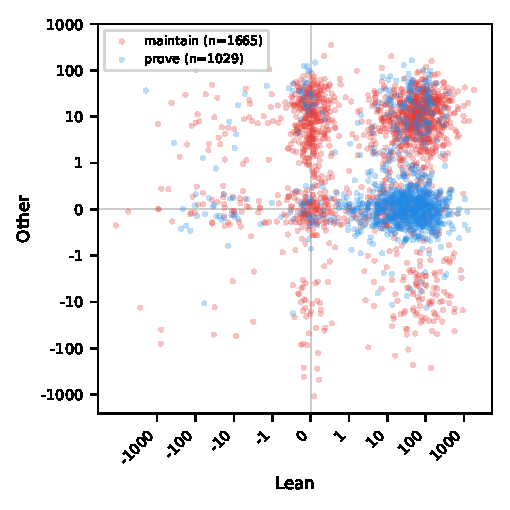
\includegraphics[width=\linewidth]{images/pr_lean_vs_other_agents.pdf}
    \subcaption{\small Net line change statistics}
    \label{fig:prover-maintainer-scatter}
  \end{subfigure}\hfill
  \begin{subfigure}[t]{0.48\linewidth}
    \centering
    \raisebox{4ex}{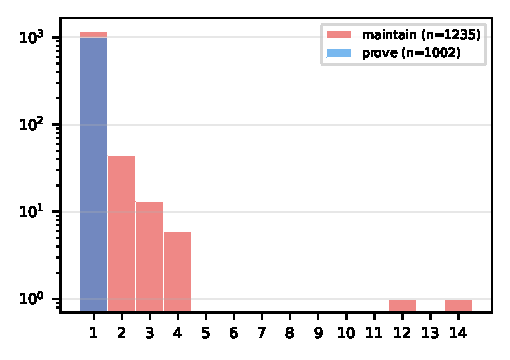
\includegraphics[width=\linewidth]{images/pr_lean_files_agents.pdf}}
    \subcaption{\small Histogram of the number of Lean files edited}
    \label{fig:prover-maintainer-hist}
  \end{subfigure}
  \caption{\textbf{Comparing prover and maintainer agents.}
    \textbf{ (a)} Net line change statistics on Lean files and coordination files (``other'') for \emph{prover} and \emph{maintainer} agents. For readability, the plot uses a symlog axis and Gaussian jitter with $\sigma = 0.3$ grid units.
    \textbf{(b)} Histogram of the number of Lean files edited for both agent types. \emph{Prover} agents work on a single file by design, \emph{maintainer} agents most frequently, too, but can also conduct large refactorings involving up to 14 files.  
  }
  \label{fig:prover-maintainer}
\end{figure}
